\section{End-to-End Testing} \label{sec:E2ETesting}
For the end-to-end testing, each of the MoSCoW requirements (Section \ref{sec:MoSCoW}) are tested manually. An overview of all the requirements and whether they were completed or not, can be found in Appendix \ref{ap:E2ETestTable}

\subsection{Must-Have}

\subsubsection{The master node must be able to receive a task from a customer} \label{sssec:mustreceivetask}
The uploading of a task from the customer page to the server is a process that goes through many files and functions in order to save the file correctly. The master node can receive a task from a customer in the system that was built.


This is done via \lstinline{router.js}, where the \lstinline{requestHandler()} function handles the request and runs the \lstinline{redirectToHandleUpload()} function. An example of file uploading is shown in figure. \ref{fig:csvFilesEmpty}, \ref{fig:uploadFileToServer} and \ref{fig:csvFilesWithUpload}

\begin{figure}[H]
    \centering
    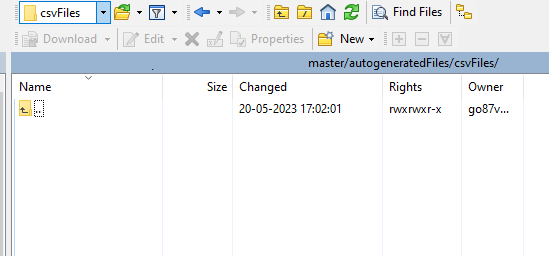
\includegraphics[scale=.5]{figures/csvFilesEmpty.png}
    \caption{The csvFiles folder empty, with no task.}
    \label{fig:csvFilesEmpty}
\end{figure}

\begin{figure}[H]
    \centering
    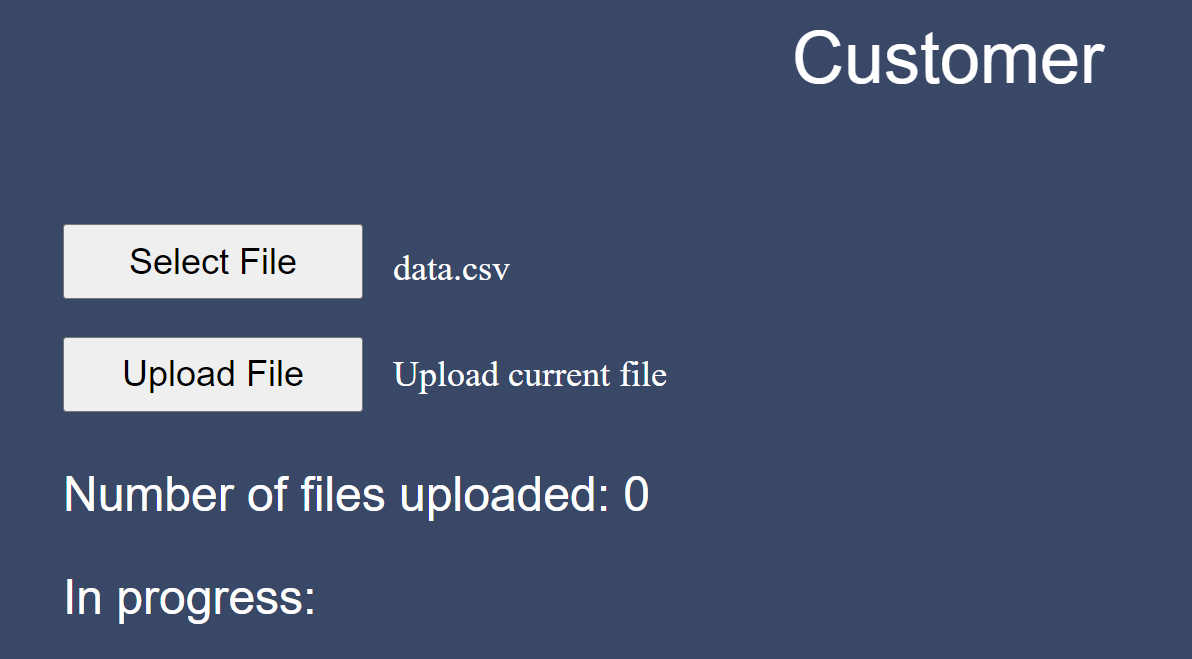
\includegraphics[scale=.5]{figures/uploadFileToServer.png}
    \caption{A task being uploaded via the customer page.}
    \label{fig:uploadFileToServer}
\end{figure}

\begin{figure}[H]
    \centering
    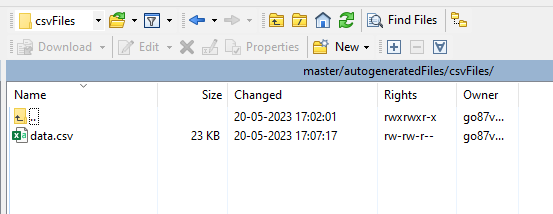
\includegraphics[scale=.5]{figures/csvFilesWithUpload.png}
    \caption{The csvFiles folder with the uploaded task.}
    \label{fig:csvFilesWithUpload}
\end{figure}


\subsubsection{The product must have a web-based user interface, where the customer can upload a CSV document, containing only numbers that need to be sorted}
This requirement is completed. The product has a user interface where the customer can upload a CSV document, containing only numbers. If a customer uploads a file that contains anything other than numbers e.g. strings or letters, the program will discard any non-number and when the customer receives the sorted file, it will only contain numbers.

\begin{figure}[H]
    \centering
    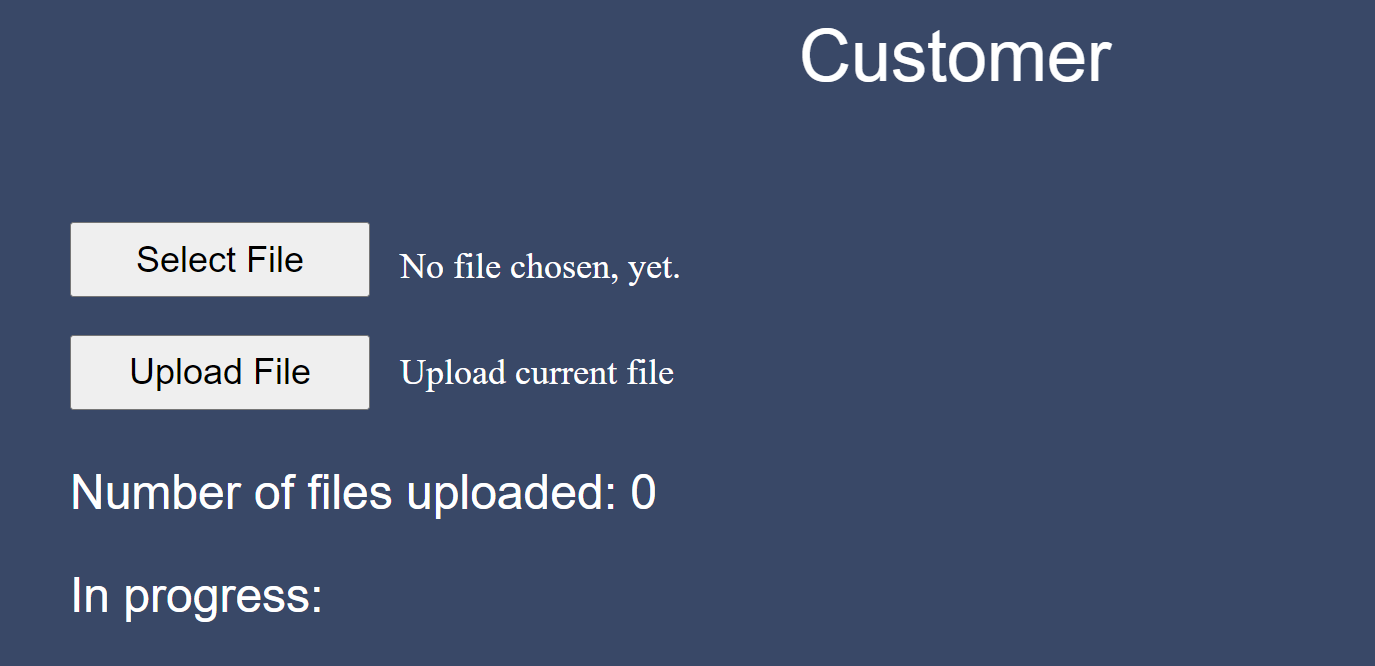
\includegraphics[scale=.3]{figures/webBasedUserInterfaceCustomer.png}
    \caption{The User interface of the customer page that handles the client side of file uploading.}
    \label{fig:my_label}
\end{figure}

\subsubsection{The master node must be able to split tasks into suitable sizes, such that any modern, consumer-grade device can be a worker node in the system} 
Splitting tasks is done by the task splitting part of the program, which is tested in a couple unit tests. The task size is controlled by a constant in the code. Currently, it is set to 100MB, which has not overwhelmed any modern machines owned by the group.

However, as mentioned in Section \ref{sub:modelSplitData}, bucket sort on a non-uniform distribution will lead to some buckets being much larger than others. This could overwhelm an older system, as the program will send these much larger buckets to a system only expecting 100MB. In this way, this requirement has not been fulfilled. However, as long as the customer mostly uploads data containing uniformly distributed values between 0 and 999,999,999, the program does fulfill the requirement. Section \ref{sec:betterBuckets} discusses how this requirement could be better fulfilled. 

\subsubsection{The master node must be able to connect, and distribute tasks, to worker nodes}
As seen on Figure \ref{fig:Distribution of Task} the worker node receives a task from the master node. This shows that the master node can connect to a worker node and assign it a task.

\begin{figure}[H]
    \centering
    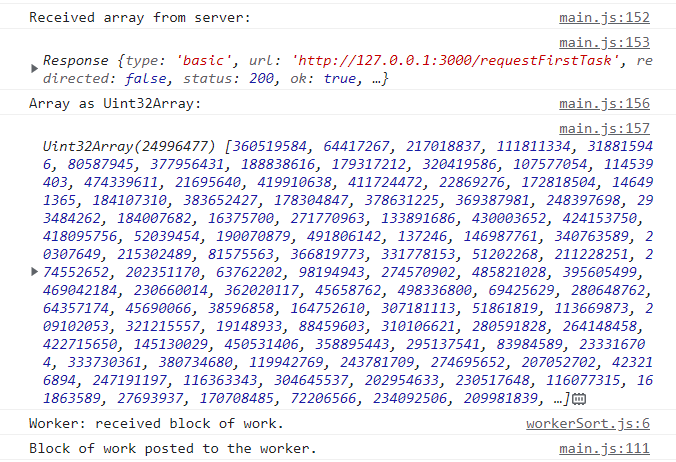
\includegraphics[scale=0.75]{figures/distributeWorkToWorker.png}
    \caption{Shown distribution of task to worker node.}
    \label{fig:Distribution of Task}
\end{figure}


\subsubsection{The grid must be able to handle a minimum of three nodes: one master and two connected worker nodes}
The master node is made using a Node.js server. The server has a request handler to communicate with workers and customers, and it keeps track of the currently active workers and assigns them tasks as they request them.

When the user loads the worker page, a UUID is generated to distinguish the node from other nodes. This allows one user to have multiple worker nodes logged into the same account and working on the same device.
When the user presses the start button on the worker interface, a request is sent to the master node, and the master node adds the worker to the list with its UUID.

\begin{figure}[H]
    \centering
    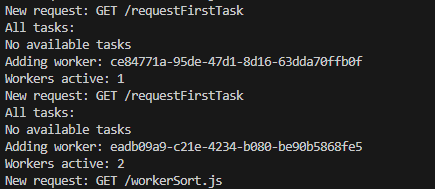
\includegraphics[scale=1]{figures/WorkersConnecting.png}
        \caption{Two workers connecting to the master node.}
    \label{fig:Workers connecting}
\end{figure}

If the worker node does not receive a task, it will wait for a few seconds before sending a new request. If the worker has not pinged the server in 20 seconds, it will automatically be removed from the list of active workers.

\begin{figure}[H]
    \centering
    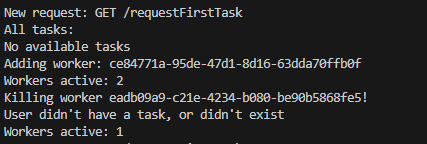
\includegraphics[scale=1]{figures/InactiveWorkerRemoved.png}
    \caption{Inactive worker is removed.}
    \label{fig:Inactive worker removed}
\end{figure}

\subsubsection{The master node must be able to receive results from worker nodes}
This requirement is achieved in the file \lstinline{main.js} through the function \lstinline{sendToServer}. The data is sent in the form of a binary octet-stream, as encoding the data in Base64 or JSON is unnecessary, wasteful, and will cause issues if the functions used are not meant to handle large amounts of data.

\begin{figure}[H]
    \centering
    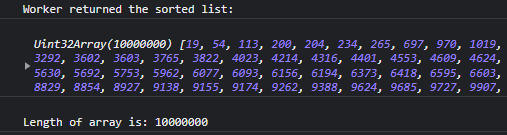
\includegraphics[scale=1]{figures/ArrayIsSent.png}
    \caption{Worker node sending results.}
    \label{fig:Sending sorted array to server}
\end{figure}

Once all the chunks of the stream have been received on the master node, they are concatenated and converted back into a \lstinline{Uint32Array}, so the sorted data is ready for use. 

\begin{figure}[H]
    \centering
    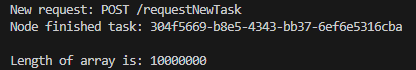
\includegraphics[scale=1.2]{figures/ReceivedArrayOnServer.png}
    \caption{Master node receiving the sorted array.}
    \label{fig:Receiving sorted array on server}
\end{figure}

\subsubsection{The master node must be able to combine results that it receives from the worker nodes}
The master node combines the sorted tasks by writing them one by one in order to a file. This file is named the same as the original file with "sorted" prepended. The sorted tasks are written to the file starting with the bucket containing the lowest values and ending with the bucket containing the highest. This results in what can be seen on Figure \ref{fig:fileSaved}, where there are two equally sized files, with the same numbers but one is sorted, while the other is not. Thereby it can be concluded that this requirement has been fulfilled. 


\begin{figure}[H]
    \centering
    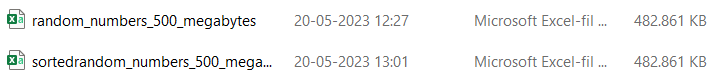
\includegraphics[scale=1]{figures/fileSaved.png}
    \caption{File before it was sorted and after.}
    \label{fig:fileSaved}
\end{figure}

\subsubsection{The master node must be able to return the final product (a sorted CSV document) to the customer}
As seen on Figure \ref{fig:fileSaved}, a new file is created with the sorted data. This sorted file can then be downloaded from the customer page using the download button shown on Figure \ref{fig:downloadFile}. This functionality fulfills the requirement.

\begin{figure}[H]
    \centering
    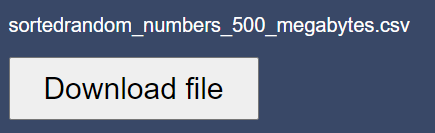
\includegraphics[scale=1]{figures/downloadFile.png}
    \caption{Download button and file name.}
    \label{fig:downloadFile}
\end{figure}

\subsection{Should-Have}

\subsubsection{The grid should be able to sort a file efficiently in regards to time} \label{sssec:timeEfficient}
To test this requirement, a file with the size of two gigabytes was uploaded to the server, split into buckets, and distributed among four worker nodes. The time was then measured and compared to the time a single computer takes to sort a file of the same size.

The time measurement starts when the file has been uploaded, and ends when all the sorted buckets are concatenated, and the data has been written onto a new CSV file. Sorting the file took 210 seconds, when using the grid computing system.

The single computer test was done on several computers in the group with varying results. The fastest computer was able to sort the file in 120 seconds, and the slowest sorted in about 300 seconds. This meant a single high quality computer could sort 90 seconds faster than the grid computing system. To figure out the cause of discrepancy, more tests were conducted.

All the relevant components of the program were timed. The sorting process for each worker, which typically involved a task with the size of 100 MB, took between 3 to 7 seconds, depending on the capabilities of the node. On a single worker, downloading the data for each task took ~21 seconds, waiting for the server to send a new task took ~9 seconds and waiting for the first task took ~16 seconds, as shown on Table \ref{tab:networkOverhead}. This finding revealed that communication overhead is a major problem in the grid. However, it is important to note that the tasks are being downloaded and sorted simultaneously, so this does not imply that the grid takes an additional 21 seconds per bucket overall.

On the master node, there are two main operations that increase the overhead. Firstly, loading the data from the uploaded file and creating buckets for different ranges of numbers takes ~63 seconds. Secondly, writing the buckets to a new file when all sorted arrays have been received takes ~61 seconds. These two factors account for 59\% of the processing time, and they alone take longer than the time it takes, for a single modern computer to sort the same task. The remaining ~86 seconds are used on sending, sorting and receiving back the data, most of which is communication overhead.

From these tests, it can be concluded that the grid, in its current state, is not able to distribute and sort tasks efficiently, and therefore this requirement is considered unaccomplished. 


\subsubsection{The master node should be able to validate the results that it receives from the worker nodes}

This requirement has not been implemented. This is a consequence of the focus in this project. Whilst result validity is significant in this kind of system, generally speaking, this project specifically focuses on time-efficient sorting on a distributed system. As such, the explicit validation of results was not implemented. However, if the unsorted file from the customer node fulfills all the given specifications for the system to run correctly, there should be no issues receiving correct, expected results. Therefore, this lack of validation is unlikely to be a problem. Alas, no guarantees are provided. 

\subsubsection{The product should have a web-based login system so that the identity of a user can be verified, to keep track of their files}
A login system was implemented in the program. This login system encompasses many different parts as described in section \ref{sec:backendLogin}. The usernames that are created by customers are utilised in the program to differentiate users. This differentiation is used in the program when the customer wants to retrieve their sorted task(s). The customer is restricted to only the task(s) that they themselves have uploaded and this restriction is implemented via their username.


\subsubsection{The master node should keep track of tasks, both tasks that are completed and pending}

The system tracks files uploaded by a customer in the CSV file named \lstinline{pendingQueue.csv}. Here, the master node keeps track of the username and the name of the file uploaded by the customer. This task is then handled when it becomes the first in the queue of pending tasks. Once the task has been completed (i.e. the file has been sorted) the file will be available for the customer to download and the information in \lstinline{pendingQueue.csv} is moved into \lstinline{finishedQueue.csv} until the customer retrieves their sorted data. As the customer completes the download of their sorted file, the completed task is removed from \lstinline{finishedQueue.csv}. 

The tracking of tasks (unsorted buckets) is handled on the master node. Specifically within \lstinline{assignWork.js}, arrays exist for tracking the pending tasks and the completed tasks. These are called, respectively, \lstinline{allTasks} and \lstinline{sortedBuckets}. The functionality surrounding these arrays is tested in the unit tests (see \lstinline{assignWork.test.js} on GitHub).

Both in terms of tracking tasks provided by the customer and tasks used in the sorting of the data, this requirement is met and satisfied.

\subsubsection{The master node should validate the type and content of the input CSV file.}
The master node validates the type of the input CSV file. However, it does not validate its content. This decision was made to focus on more important features, as the lack of validation of the contents of the CSV file does not interfere with the sorting process, as letters and strings, that might be included in the file, will simply be discarded. While it may be a problem that the content is not validated, as long as the CSV file that is uploaded has the right requirements then it should still yield the correct result. 

\begin{figure} [H]
    \centering
    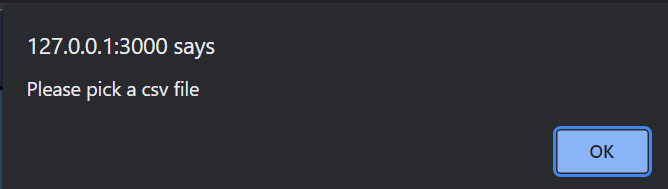
\includegraphics[scale=.75]{figures/fileMustBeCSV.png}
    \caption{The alert message when a customer tries to upload a non-CSV file.}
    \label{fig:fileMustBeCSV}
\end{figure}
\subsection{Could-Have}

\subsubsection{Login sessions could expire after some time, in order to enhance security}

This requirement has not been fulfilled but to enhance security within the system, the login function could utilise web tokens, to give the users a session with a fixed time to live.

The implementation of access tokens has already been achieved, thereby laying the foundation for this function to be completed. Upon login, an access token is sent to the client-side, and this is then sent upon entering the protected resources, such as the worker page, and customer page.
Applying a fixed time for access tokens to be valid, would require the user to log in again, once the time limit is reached. If an access token were to be intercepted, a fixed time for its validity would limit the use of this access token.
Since the system currently does not make use of HTTPS, nor a fixed time limit for access tokens, an intercepted token would not need to be decrypted, and can forever be misused to impersonate other users.

\subsubsection{The login system could have a mechanism for preventing SQL injections and similar attacks}
There was no explicit effort made to protect the program against SQL injections or similar attacks, since the project does not focus on the security of the program. The library better-sqlite3 that was used does, however, claim to have some innate protections against these types of attacks \cite{SQLInjectionsBettersqlite3}. Nonetheless, since this claim cannot be confirmed, the requirement is considered unfulfilled.

\subsubsection{There could be a reward system for contributing worker nodes}
This requirement was not fulfilled by the program. While a reward system for workers would motivate workers to give computational power, such a system was left out. This feature is not a necessity for the program but instead a feature that would enhance the user experience. It was therefore decided that it should be left out, since this project does not especially focus on user experience.


\subsection{Will-Not-Have}
None of the \emph{will not have} requirements have been made as it was already determined in the beginning that these two requirements are not possible given the time frame of the project. While they were not intended to be made, they still serve as possible future development features as they can still be relevant for the system. The two \emph{will not have} requirements are as follows:
\begin{itemize}
      \item The master node will not be able to process two files simultaneously.
      \item The frontend will not have an option for the customer to upload custom scripts for workers to run.
  \end{itemize}
